\section{Исследование управляемости}

Рассматриваем систему:
\begin{equation*}
    \dot x=Ax+Bu,\quad
    A=\begin{bmatrix}
        -1 & 1 & 0 \\ -2 & -4 & -1 \\ 2 & 2 & -1
    \end{bmatrix},\quad
    B=\begin{bmatrix}
        2 \\ 3 \\ -1
    \end{bmatrix},\quad
    x_1=\begin{bmatrix}
        1 \\ -3 \\ 3
    \end{bmatrix}.
\end{equation*}

\subsection{Исследование управляемости}

Найдем матрицу управляемости:
\begin{equation*}
    U=[B\quad AB\quad A^2B]=
    \begin{bmatrix}
        2 & 1 & -16 \\ 3 & -15 & 47 \\ -1 & 11 & -39
    \end{bmatrix}.
\end{equation*}
Матрица полноранговая, следовательно \textbf{система управляема}.

Спектр матрицы $A$:
$$\sigma(A)=\{ -2 + j; -2-j; -2\},$$
тогда матрицы Хаутуса ($[A-\lambda_iI\quad B]$) соответственно:
\begin{equation*}
    \begin{bmatrix}
        1-j&1&0&2\\-2&-2-j&-1&3\\2&2&1-j&-1
    \end{bmatrix},\quad 
    \begin{bmatrix}
        1+j&1&0&2\\-2&-2+j&-1&3\\2&2&1+j&-1
    \end{bmatrix},\quad
    \begin{bmatrix}
        1 & 1 & 0 & 2 \\
        -2 & -2 & -1 & 3 \\
        2 & 2 & 1 & -1
    \end{bmatrix}.
\end{equation*}
Все они трехранговые, \textbf{что удовлетворяет критерию Хаутуса управляемой системы}.

Жорданова форма матрицы $A$ и $P^{-1}B$:
\begin{equation*}
    A =\begin{bmatrix}
        
-2&	   0&	   0\\
0&	  -2&	   -1\\
0&	   1&	  -2\\

    \end{bmatrix},\quad
    P^{-1}B=\begin{bmatrix}
        2.0000 \\ -0.7071 \\ -6.3640
    \end{bmatrix}.
\end{equation*}
Как видно, система в Жордановой форме полностью управляема, а значит и \textbf{исходная система
полностью управляема}.

Итого, все три критерия сошлись на том, что система полностью управляема.

\subsection{Грамиан}

Найдем Грамиан управляемости системы относительно времени $t_1=3$:
\begin{equation*}
    P(3)=\int_{0}^{3}e^{At}BB^Te^{A^Tt}dt=
    \begin{bmatrix}
        2.2838  &  0.2838  &  1.1868 \\
        0.2838   & 1.1735  & -0.7618 \\
        1.1868  & -0.7618  &  1.3500
    \end{bmatrix}.
\end{equation*}
Его спектр:
\begin{equation*}
    \sigma(P(3))=\{ 0.0034;\ 
    3.1144;\ 
    1.6894\},
\end{equation*}
все числа положительны, а значит $det(P(3))=\lambda_1\cdot\lambda_2\cdot\lambda_3>0$ и
можно найти управление, которое переводит систему которое переводит систему из $x(0)=0$ в $x(3) = x_1$.

\subsection{Управление}

Чтобы перевести систему из $x(0)=0$ в $x(3)=x_1$, достаточно взять программное управление:
\begin{multline*}
    u(t) = B^T e^{A^T(3 - t)} P(3)^{-1} x_1 = \\ =
    \begin{bmatrix}
        2 & 3 & -1
    \end{bmatrix}\cdot
    \exp\left( \begin{bmatrix}
        -1 & -2 & 2 \\ 
         1 & -4 & 2 \\ 
         0 & -1 & -1
    \end{bmatrix}\cdot(3 - t) \right)\cdot
    \begin{bmatrix}
        2.2838  &  0.2838  &  1.1868 \\
        0.2838   & 1.1735  & -0.7618 \\
        1.1868  & -0.7618  &  1.3500
    \end{bmatrix}^{-1}
    \begin{bmatrix}
        1 \\ -3 \\ 3
    \end{bmatrix}=\\
    =\begin{bmatrix}
        2 & 3 & -1
    \end{bmatrix}\cdot
    \begin{bmatrix}
        -1.0000&    0.7071 &  -0.7071\\
        1.0000  & -1.4142 &        0\\
             0   & 1.4142&         0
    \end{bmatrix}\cdot
    \begin{bmatrix}
        e^{-2(3-t)}&     0 &    0\\
        0  &  e^{-2t}\cos(3-t) &   e^{-2t}\sin(3-t)  \\
        0   &  -e^{-2t}\sin(3-t)&    e^{-2t}\cos(3-t) \\
    \end{bmatrix}\cdot\\
    \cdot\begin{bmatrix}
        0&    1.0000  &  1.0000\\
        0 &        0 &   0.7071\\
  -1.4142  & -1.4142&   -0.7071\\
    \end{bmatrix}\cdot
    \begin{bmatrix}
        55.6117&  -71.3016  &-89.1208\\
        -71.3016&   92.7627 & 115.0234\\
        -89.1208 & 115.0234&  143.9898\\
    \end{bmatrix}\cdot
    \begin{bmatrix}
        1 \\ -3 \\ 3
    \end{bmatrix}=\\
    =\begin{bmatrix}
        1 & -4.243 & -1.414
    \end{bmatrix}\cdot
    \begin{bmatrix}
        e^{-2(3-t)}&     0 &    0\\
        0  &  e^{-2t}\cos(3-t) &   e^{-2t}\sin(3-t)  \\
        0   &  -e^{-2t}\sin(3-t)&    e^{-2t}\cos(3-t) \\
    \end{bmatrix}\cdot\\
    \cdot\begin{bmatrix}
        -160.422 & 207.786 & 259.013\\
        -63.017 & 81.333 & 101.815\\
        85.206 & -111.683 & -138.447
    \end{bmatrix}\cdot
    \begin{bmatrix}
        1 \\ -3 \\ 3
    \end{bmatrix}=\\
    =\begin{bmatrix}
        e^{-2(3-t)} \\ e^{-2t}[1.414\sin(3-t)-4.243\cos(3-t)] \\ -e^{-2t}[1.414\cos(3-t)+4.243\sin(3-t)]
    \end{bmatrix}^T
    \cdot\begin{bmatrix}
        -6.741 \\ -1.571 \\ 4.916
    \end{bmatrix}=\\
    =-6.741e^{-2(3-t)}-1.571e^{-2t}[1.414\sin(3-t)-4.243\cos(3-t)]-4.916e^{-2t}[1.414\cos(3-t)+4.243\sin(3-t)].
\end{multline*}

Смоделируем систему и данное управление, результаты приведены на рисунке \ref{fig:task1}.
\begin{figure}[H]
    \centering
    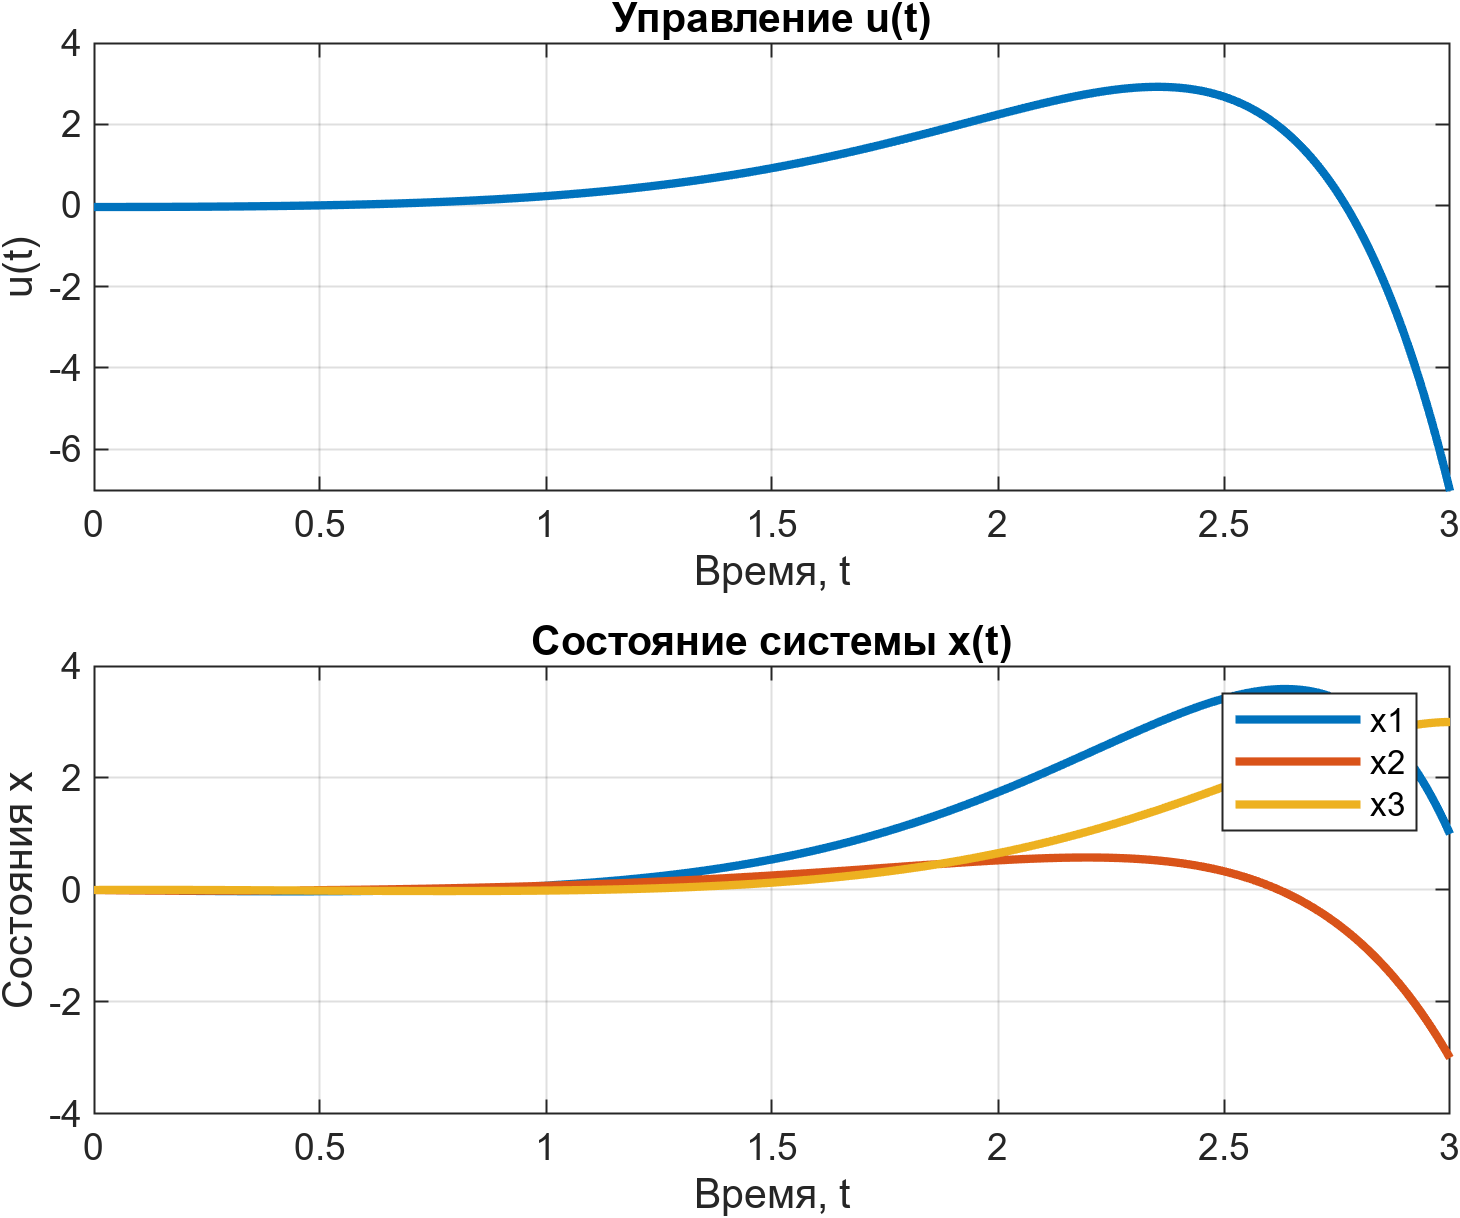
\includegraphics[width=0.7\textwidth]{figs/task_1.png}
    \caption{Система с программным управлением}
    \label{fig:task1}
\end{figure}
Как видно, система переводится в состояние $x_1$ за время $t_1=3$.
В итоге, по всем критериям система управляема и управление найдено.



\section{Еще одно исследование управляемости}

Рассматриваем систему:
\begin{equation*}
    \dot x=Ax+Bu,\quad
    A=\begin{bmatrix}
        -1 & 1 & 0 \\ -2 & -4 & -1 \\ 2 & 2 & -1
    \end{bmatrix},\quad
    B=\begin{bmatrix}
        2 \\ -1 \\ 1
    \end{bmatrix},\quad
    x_1'=\begin{bmatrix}
        1 \\ -3 \\ 3
    \end{bmatrix},\quad
    x_1''=\begin{bmatrix}
        0\\-2\\3
    \end{bmatrix}.
\end{equation*}

\subsection{Проверка точек}

Если состояние $x_1$ принадлежит управляемому множеству, то
\begin{equation*}
    rank\ U=rank\ [U\ x_1].
\end{equation*}
Проверим данные состояния $x_1'$ и $x_1''$:
\begin{equation*}
    [U\ x_1']=
    \begin{bmatrix}
        2 & -3 & 2 & 1\\
        -1 & -1 & 9 & -3\\
        1 & 1 & -9 & 3
    \end{bmatrix};\quad
    [U\ x_1'']=
    \begin{bmatrix}
        2 & -3 & 2 & 0\\
        -1 & -1 & 9 & -2\\
        1 & 1 & -9 & 3
    \end{bmatrix}.
\end{equation*}
Первая матрица имеет ранг 2, а вторая 3. Если посмотреть чуть ниже на ранг матрицы управляемости,
то делаем вывод, что только $x_1'$ принадлежит управляемому пространству. Это состояние будет
целевым $x_1=x_1'$.

\subsection{Исследование управляемости}

Найдем матрицу управляемости:
\begin{equation*}
    U=[B\quad AB\quad A^2B]=
    \begin{bmatrix}
        2 & -3 & 2 \\ -1 & -1 & 9 \\ 1 & 1 & -9
    \end{bmatrix}.
\end{equation*}
Матрица имеет ранг 2, следовательно \textbf{система не управляема}.

Спектр матрицы $A$:
$$\sigma(A)=\{ -2 + j;\ -2-j;\ -2\},$$
тогда матрицы Хаутуса ($[A-\lambda_iI\quad B]$) соответственно:
\begin{equation*}
    \begin{bmatrix}
        1-j&1&0&2\\
        -2&-2-j&-1&-1\\
        2&2&1-j&1
    \end{bmatrix},\quad 
    \begin{bmatrix}
        1+j&1&0&2\\-2&-2+j&-1&-1\\2&2&1+j&1
    \end{bmatrix},\quad
    \begin{bmatrix}
        1 & 1 & 0 & 2 \\
        -2 & -2 & -1 & -1 \\
        2 & 2 & 1 & 1
    \end{bmatrix}.
\end{equation*}
Первые две матрицы трехранговые, что делает комплексно сопряженные корни
\textbf{управлемыми}, но а вот третья матрица имеет ранг 2, следовательно собственное
число $-2$ \textbf{не управляемо}. Значит система не управлема.

Жорданова форма матрицы $A$ и $P^{-1}B$:
\begin{equation*}
    A =\begin{bmatrix}
        
-2&	   0&	   0\\
0&	  -2&	   -1\\
0&	   1&	  -2\\

    \end{bmatrix},\quad
    P^{-1}B=\begin{bmatrix}
        0 \\ 0.7071 \\ -2.1213
    \end{bmatrix}.
\end{equation*}
Как видно, одна из клеток не управляема, а значит и \textbf{исходная система
не управляема}.

Итого, все три критерия сошлись на том, что система не управляема.

\subsection{Грамиан}

Найдем Грамиан управляемости системы относительно времени $t_1=3$:
\begin{equation*}
    P(3)=\int_{0}^{3}e^{At}BB^Te^{A^Tt}dt=
    \begin{bmatrix}
        1.1250  & -0.8750   & 0.8750\\
        -0.8750  &  0.7500 &  -0.7500\\
         0.8750   &-0.7500&    0.7500
    \end{bmatrix}.
\end{equation*}
Его спектр:
\begin{equation*}
    \sigma(P(3))=\{ 2.5640;\ 
    0.0609;\ 
    0.0000\},
\end{equation*}
одно число нулевое, а значит Грамиан вырожден и программное управление честно найти не представлется
возможным. Будем использовать псевдообратную матрицу:
\begin{equation*}
    P(3)^+=\begin{bmatrix}
        9.6001&    5.6001  & -5.6001\\
        5.6001 &   3.6000 &  -3.6000\\
       -5.6001  & -3.6000&    3.6000
    \end{bmatrix}.
\end{equation*}

\subsection{Управление}

Чтобы перевести систему из $x(0)=0$ в $x(3)=x_1$, возьмем программное управление:
\begin{multline*}
    u(t) = B^T e^{A^T(3 - t)} P(3)^+ x_1 = \\ =
    \begin{bmatrix}
        2 & -1 & 1
    \end{bmatrix}\cdot
    \begin{bmatrix}
        -1.0000&    0.7071 &  -0.7071\\
        1.0000  & -1.4142 &        0\\
             0   & 1.4142&         0
    \end{bmatrix}\cdot
    \begin{bmatrix}
        e^{-2(3-t)}&     0 &    0\\
        0  &  e^{-2t}\cos(3-t) &   e^{-2t}\sin(3-t)  \\
        0   &  -e^{-2t}\sin(3-t)&    e^{-2t}\cos(3-t) \\
    \end{bmatrix}\cdot\\
    \cdot\begin{bmatrix}
        0&    1.0000  &  1.0000\\
        0 &        0 &   0.7071\\
  -1.4142  & -1.4142&   -0.7071\\
    \end{bmatrix}\cdot
    \begin{bmatrix}
        9.6001&    5.6001  & -5.6001\\
        5.6001 &   3.6000 &  -3.6000\\
       -5.6001  & -3.6000&    3.6000
    \end{bmatrix}
    \begin{bmatrix}
        1 \\ -3 \\ 3
    \end{bmatrix}=\\
    =\begin{bmatrix}
        -3 & 4.243 & -1.414
    \end{bmatrix}\cdot
    \begin{bmatrix}
        e^{-2(3-t)}&     0 &    0\\
        0  &  e^{-2t}\cos(3-t) &   e^{-2t}\sin(3-t)  \\
        0   &  -e^{-2t}\sin(3-t)&    e^{-2t}\cos(3-t) \\
    \end{bmatrix}\cdot
    \begin{bmatrix}
        0 \\ 11.314 \\ 45.255
    \end{bmatrix}=\\
    =\begin{bmatrix}
        -3 & 4.243 & -1.414
    \end{bmatrix}\cdot
    \begin{bmatrix}
        0 \\ e^{-2t}[11.314\cos(3-t)+45.255\sin(3-t)] \\ e^{-2t}[45.255\cos(3-t)-11.314\sin(3-t)]
    \end{bmatrix}=\\
    =e^{-2t}\Big( 208.015\sin(3-t) - 15.985\cos(3-t) \Big).
\end{multline*}
Смоделируем систему и данное управление, результаты приведены на рисунке \ref{fig:task2}.
\begin{figure}[H]
    \centering
    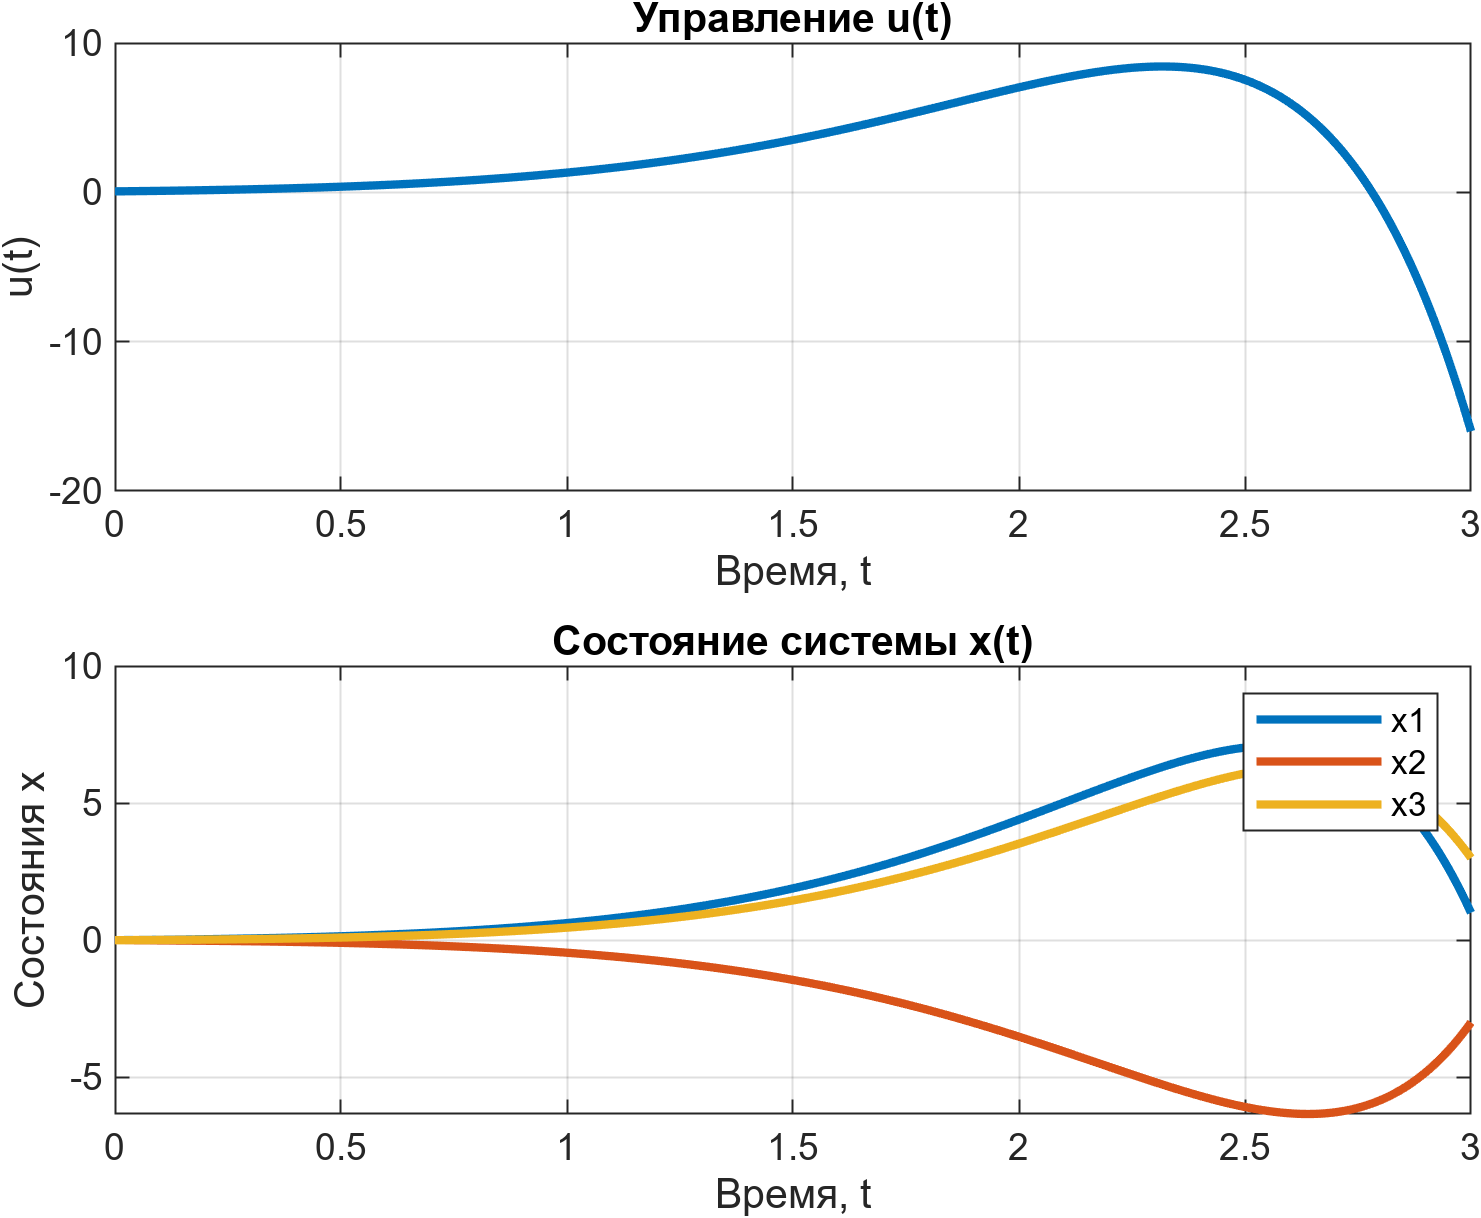
\includegraphics[width=0.7\textwidth]{figs/task_2.png}
    \caption{Система с "псевдо программным" управлением}
    \label{fig:task2}
\end{figure}
Как видно, система переводится в состояние $x_1$ за время $t_1=3$.
В итоге, по всем критериям система не управляема, но для состояния из
управляемого пространства было найдено управление.


\section{Исследование наблюдаемости}
